\section{Numerische Lösung}
\rhead{Numerische Lösung}

Die El-Niño-DDE soll mithilfe von Matlab numerisch gelöst werden.
Matlab stellt zum Lösen von DDEs eine fertige Funktion zu Verfügung (\texttt{dde23}).
Da diese Funktion auf anderen Systemen (z.B. Octave) nicht verwendbar ist, soll eine eigene Lösungsfunktion geschrieben werden.
Beim Schreiben dieser Funktion wird darauf geachtet, dass die Syntax mit \texttt{dde23} vergleichbar ist. 

\subsection{Analyse der Funktion \texttt{dde23}}
Die offizielle Syntax von \texttt{dde23} \footnote{https://www.mathworks.com/help/matlab/ref/dde23.html} lautet: 
\begin{lstlisting}[style=MATLAB]{dde23}
	sol = dde23(ddefun,lags,history,tspan);
\end{lstlisting}
Wir analysieren zunächst alle Parameter.

\subsubsection{Parameter: \texttt{ddefun}}
Die \texttt{ddefun} stellt die eigentliche DDE dar, welche als Funktion übergeben werden muss.
Unsere El-Niño-DDE \eqref{eldde} hat als eigene Parameter die Zeit (t), den aktuellen Wert (y), die verzögerten Werte (Z) und alle Konstanten.
\begin{lstlisting}[style=MATLAB]{dde_full}
	function dydt = dde_full(t,y,Z,c,a,b,e)
	ylag1 = Z(:,1);
	ylag2 = Z(:,2);
	dydt = -c*y+a*ylag1-b*ylag2-e*y.^3;
\end{lstlisting}
Damit diese Funktion akzeptiert wird, müssen die Konstanten gesetzt werden.
\begin{lstlisting}[style=MATLAB]{my_dde}
	c = 1; a = 2.6; b = 3; e = 0.1;
	my_dde = @(t,y,Z) dde_full(t,y,Z,c,a,b,e);
\end{lstlisting}

\subsubsection{Parameter: lags}
Die Verzögerungen (in Jahren) entsprechen einem simplen Vektor.
\begin{lstlisting}[style=MATLAB]{lags}
	tauk = 0.15; taur = 1;
	tau = [0.5*tauk 0.5*taur+tauk];
\end{lstlisting}

\subsubsection{Parameter: history}
Die history entspricht einer Funktion, welche die Werte aus der Vergangenheit ausgibt. 
Das kann mit Vektoren (mit realen Daten\footnote{http://www.cpc.ncep.noaa.gov/data/indices/sstoi.indices}) und einer Interpolation gelöst werden.
\begin{lstlisting}[style=MATLAB]{hist}
	function s = dde_hist(t)
	t_v = [-0.67,-0.58,-0.5,-0.42, ...];
	s_v = [0.71,0.5,-0.06,-0.4,...];  
	s = @(t) interp1(t_v,s_v,t);
\end{lstlisting}

\subsubsection{Gesamte Anwendung}
Der Parameter \texttt{tspan} gibt die zu berechnende Zeitspanne (hier 0-3 Jahre) an.
\begin{lstlisting}[style=MATLAB]{Anwendung}
	sol = dde23(my_dde,tau,dde_hist,[0, 3]);
\end{lstlisting}
Der Aufruf \texttt{dde23} soll nun durch eine eigene Funktion ersetzt werden.
 

\subsection{Berchnung von endlich kurzen Zeitschritten}
Bei diesem Ansatz wird immer die Ableitung zu einer bestimmten Zeit berechnet.
Diese Ableitung wird dann für einen (kurzen) Zeitschritt als Konstant genommen und damit nächste Wert berechnet.
\begin{algorithm}
	\caption{Numerischer DDE-Solver}
	\label{algo1}
	\begin{algorithmic}[1]
		\State Initialisieren, d.h. Zeitachse erstellen, Zeitschritt dt berechnen, etc
		\For{dt in t}
		\State Bestimmen ob die verzögerten Werte dde\_hist oder in alter Lösung (wenn t > $\tau$) vorkommen
		\For{i in tau}
		\State Korrekten verzögerten Wert für jedes $\tau$ finden
		\EndFor
		\State dde-Funktion aufrufen und dydt speichern
		\State Nächster Wert = aktueller Wert + dydt*dt
		\EndFor
	\end{algorithmic}
\end{algorithm}

Mit diesem Algorithmus wird ein identisches Ergebnis wie mit \texttt{dde23} erreicht (vgl. Abbildung \ref{fig:vgl_dde23}). 
\begin{figure}
	\centering
	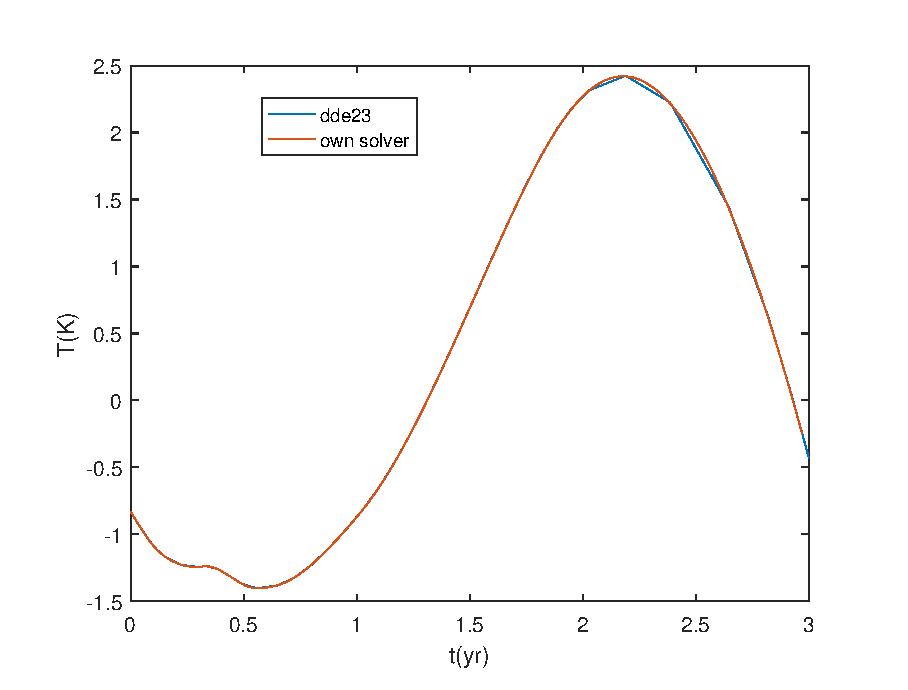
\includegraphics{verzoegert/inp/figures/vgl_dde23.eps}
	\caption{Vergleich der eigenen Lösungsfunktion mit dde23}
	\label{fig:vgl_dde23}
\end{figure}
Es werden jeweils 10000 Datenpunkte berechnet. 
Bei mehr Datenpunkten dauert die Berechnung sehr lange, wohl auch weil der Algorithmus nicht optimiert ist.

\subsection{Instabilität bei wenigen Datenpunkten} \label{num:instabil}
Der Algorithmus von \texttt{dde23} berechnet viel weniger Datenpunkte.
Wenn wir die Anzahl Datenpunkte in unserem Algorithmus reduzieren, werden die Lösungen schnell instabil (vgl. Abbildung \ref{fig:instab100}).
\begin{figure}
	\centering
	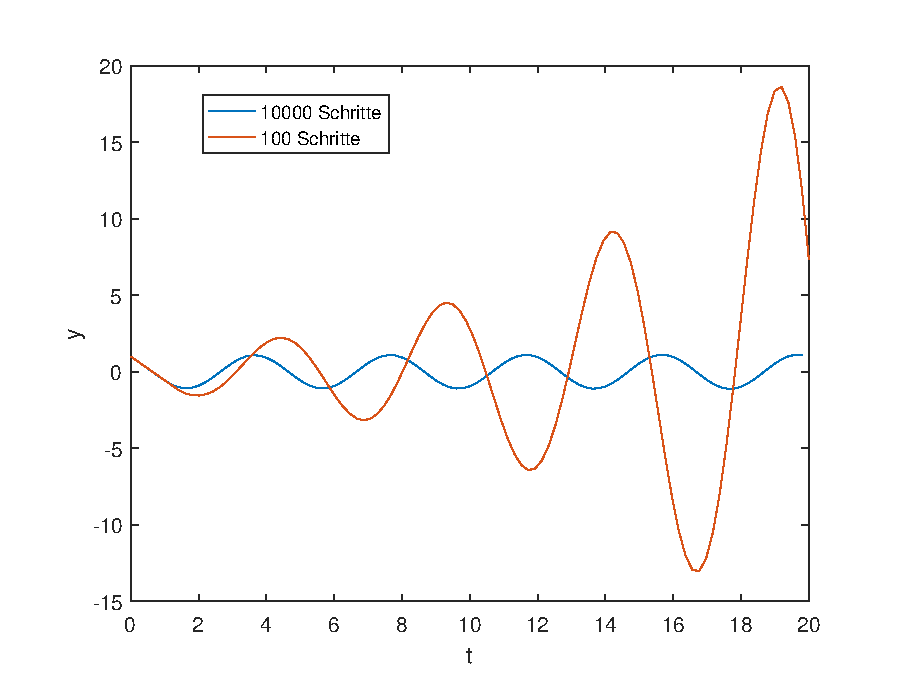
\includegraphics{verzoegert/inp/figures/instab100.eps}
	\caption{Vergleich der Lösung mit 10000 Datenpunkten und der Lösung mit 100 Datenpunkten. Gelöst wurde das Beispiel von \eqref{bsp}.}
	\label{fig:instab100}
\end{figure}
Auf den ersten Blick scheint dieses Resultat verblüffend, da 100 Datenpunkte immer noch relativ viel sind.

\subsubsection{title}
%todo Wieso gibt es dieses Phänomen...erklären